\documentclass[a5paper,12pt]{memoir}
\usepackage{fontspec}
\usepackage[top=-10mm,left=10mm,bottom=30mm,right=10mm]{geometry}
\usepackage{multicol}
\usepackage{setspace}
\usepackage{xeCJK}
\usepackage{wrapfig}
\usepackage{graphicx}
\pagestyle{empty}
\graphicspath{{./images/}}
\newcommand*\CJKmovesymbol[1]{\raise.35em\hbox{#1}}
\newcommand*\CJKmove{\punctstyle{plain}
		       \let\CJKsymbol\CJKmovesymbol
			   \let\CJKpunctsymbol\CJKsymbol}
\setmainfont{Noto Serif CJK KR}
\setCJKmainfont{Noto Serif CJK KR}
\newcommand{\CJKnumber}[1]{{#1}}
\newcommand{\explain}[2]{{$\bullet$}〔{#1}〕{#2}}
\newcommand{\go}[2]{\\{$\bullet$}請考\textbf{#2}。 }
\newcommand{\entry}[4]{{\par\nopagebreak{{\vspace{1.5mm}{\bfseries{#1}}{\textsuperscript{\CJKnumber{#2}}}{#3}}}}}
\newcommand{\also}[1]{\\亦曰\textbf{#1}。}
\newcommand{\samp}[2]{{#1}曰:『{#2}』}
\newcommand{\syn}[2]{通\textbf{#1}\textsuperscript{\CJKnumber{#2}}。}
\newcommand{\ant}[2]{對\textbf{#1}\textsuperscript{\CJKnumber{#2}}。}
\begin{document}
\linespread{1.25}
\begin{wrapfigure}{r}{60mm}
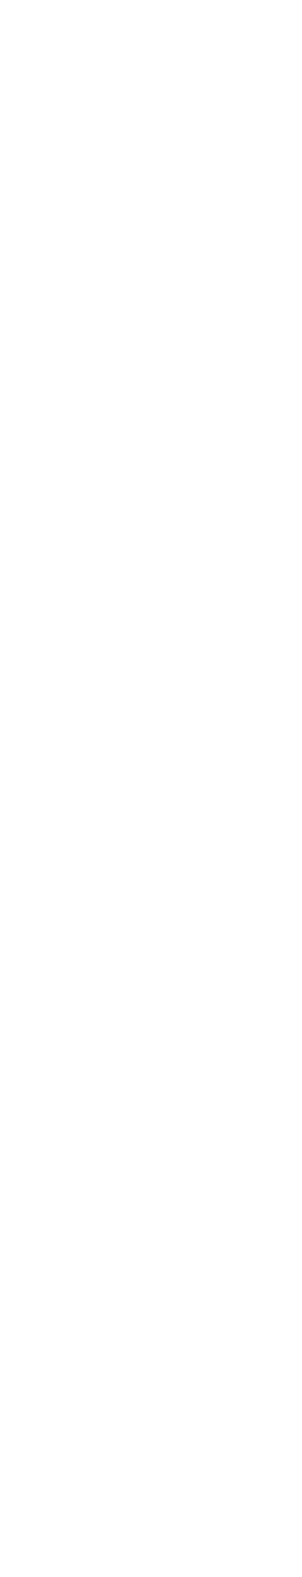
\includegraphics[height=220mm]{cover.png}
\end{wrapfigure}
\hfill
\vfill
{\HUGE{漢詞林}}\\
{李世鎬\hspace{14pt}編著}
\vspace{64pt}
\frontmatter
\newpage
\addtolength{\topmargin}{20mm}
\linespread{1.25}
\section{序}
華夏、雞林、扶桑之類、古以漢文爲國風之礎矣。
古欲習漢文、以字典爲寶。
字典雖有文字之解、未有詞彙之解。
各國、雖有其辭書者、以諺解漢。
他國之人視、畫中之餅也耳。
以漢解漢、四海蒼生之習漢文者、皆可以讀。
余願此書爲江湖諸賢所補、爲四海諸學所寶耳。
\section{範例}
此書之範例如左。
\par 第一條:「各項、取諸漢文古典、順之若康熙字典。」
\par 第二條:「諺字與邦字、載而明之。」
\par 第三條:「詞之常同而綴之者、亦載之矣。」
\par 第四修:「變品之事、若從常道、不之載。」

\mainmatter
\linespread{1.17}
\begin{multicols}{3}
\input{hcl-entries.tex}
\end{multicols}
\appendix
\newpage
\section{所考文章}
Hornby, A S. "Oxford Advanced Learner's Dictionary." 9th Edition, Oxford University Press, 2015, Oxford. \\
김종호(金琮鎬). "한문 해석 공식: 촘스키가 논어를 읽는다면." 한티미디어, 2019, 서울.

\end{document}
